\section{Thực nghiệm và kết quả}

\textit{A. Dữ liệu}

\begin{table*}[t]
\centering
\caption{Kết quả đánh giá tổng hợp: phân loại tư thế gắn kết (I) và dự đoán ái lực liên kết (II). GNINA-D18/GNINA-Ds = GNINA Default2018/Dense; R+/R\texttt{-} = recall lớp tư thế tốt/xấu.}
\label{tab:combined_results}
\footnotesize
\begin{tabular}{lc ccccc ccccc}
\hline
\multirow{2}{*}{\textbf{Mô hình}} & \multirow{2}{*}{\textbf{Params}} & \multicolumn{5}{c}{\textbf{I. Phân loại tư thế}} & \multicolumn{5}{c}{\textbf{II. Dự đoán ái lực}} \\
\cmidrule(lr){3-7} \cmidrule(lr){8-12}
 & & Acc & BalAcc & R+ & R\texttt{-} & PR-AUC & MAE & RMSE & $r$ & $\rho$ & C-idx \\
\hline
\textbf{GNINA-D18}     & 2.16M & 0.627 & 0.761 & \textbf{0.945} & 0.578 & 0.486 & 1.046 & 1.381 & 0.775 & 0.766 & 0.793 \\
\textbf{GNINA-Ds}      & 0.46M & 0.761 & 0.787 & 0.823          & 0.751 & 0.510 & \textbf{1.026} & \textbf{1.324} & \textbf{0.799} & \textbf{0.784} & \textbf{0.801} \\
\textbf{Pafnucy}       & 7.99M & 0.689 & 0.790 & 0.928          & 0.652 & 0.562 & 1.149 & 1.417 & 0.768 & 0.756 & 0.782 \\
\textbf{GeoFormerDock} & 1.59M & \textbf{0.814} & \textbf{0.830} & 0.851 & \textbf{0.808} & \textbf{0.631} & 1.221 & 1.525 & 0.752 & 0.732 & 0.771 \\
\hline
\end{tabular}
\end{table*}

Thực nghiệm sử dụng tập CrossDocked2020~\cite{francoeur2020three}, chia theo split \texttt{ref\_uff} do chính nhóm tác giả bộ dữ liệu công bố kèm bản phát hành (không phải bộ lọc tự chọn của nghiên cứu này): 62.335 mẫu huấn luyện và 4.618 mẫu kiểm tra, trong đó 623 mẫu (13.5\%) có nhãn ái lực dương (mẫu thực nghiệm), số còn lại là decoy. Cả hai tập đều được chuyển thành lưới voxel $28 \times 48 \times 48 \times 48$ với cùng quy trình mô tả ở Mục III.A; phép tăng cường (xoay ngẫu nhiên, tịnh tiến $\pm 1.0$ \AA) chỉ áp dụng cho tập huấn luyện.

\textit{B. Thiết lập thực nghiệm}

Pafnucy và hai mô hình GNINA được cài đặt lại, huấn luyện từ đầu dưới cùng biểu diễn voxel $28\times48^3$ và cùng các siêu tham số tối ưu hóa chính (AdamW, $10^{-3}$, 100 epoch, Mục III.C), nên số liệu phản ánh năng lực kiến trúc dưới điều kiện biểu diễn chung, không phải kết quả đã công bố nguyên bản. Hai mô hình GNINA dùng hàm hồi quy Gaussian NLL dị phương sai thay vì Huber, một khác biệt cần lưu ý khi diễn giải hiệu năng ở nhánh ái lực (Mục IV.D). Đối với nhánh phân loại tư thế của GeoFormerDock được huấn luyện với cân bằng lớp ở mức minibatch (32 mẫu tốt/32 mẫu xấu mỗi batch). Mô hình tốt nhất của mỗi kiến trúc được chọn theo chỉ số tổng hợp trên chính tập kiểm tra; một phép chọn đối chứng bằng chỉ số trên tập huấn luyện cho thứ hạng tương đối nhất quán giữa các mô hình.


\textit{C. Kết quả chính}

Bảng~\ref{tab:combined_results} cho thấy GeoFormerDock dẫn đầu rõ rệt ở nhánh phân loại tư thế, còn ở nhánh ái lực khoảng cách với baseline không đồng đều giữa các mô hình. Xét theo từng lớp, GeoFormerDock đạt R\texttt{-}=0.808 (nhận diện tư thế nhiễu), cao hơn so với GNINA-D18 (0.578) và Pafnucy (0.652), đổi lại R+=0.578 giảm nhẹ so với hai mô hình này (0.945 và 0.928 tương ứng). Kết quả này phản ánh hiệu quả của cân bằng lớp ở mức minibatch (Mục IV.B) và cho thấy mô hình nhận diện đồng đều hơn thay vì thiên lệch về tư thế tốt như các baseline. So sánh cặp có kiểm định (paired bootstrap, $n=2000$, $\alpha=0.05$) cho thấy GeoFormerDock so với GNINA Dense, mô hình dùng hàm hồi quy Gaussian NLL thay vì Huber như các mô hình còn lại, khác biệt có ý nghĩa thống kê trên cả 5 chỉ số; so với GNINA Default2018 và Pafnucy, khác biệt có ý nghĩa chủ yếu ở MAE/RMSE, trong khi Pearson/Spearman/C-index đều có khoảng tin cậy chứa 0, chưa đủ bằng chứng kết luận có khác biệt về các chỉ số tương quan và xếp hạng ái lực.

\begin{figure}[H]
    \centering
    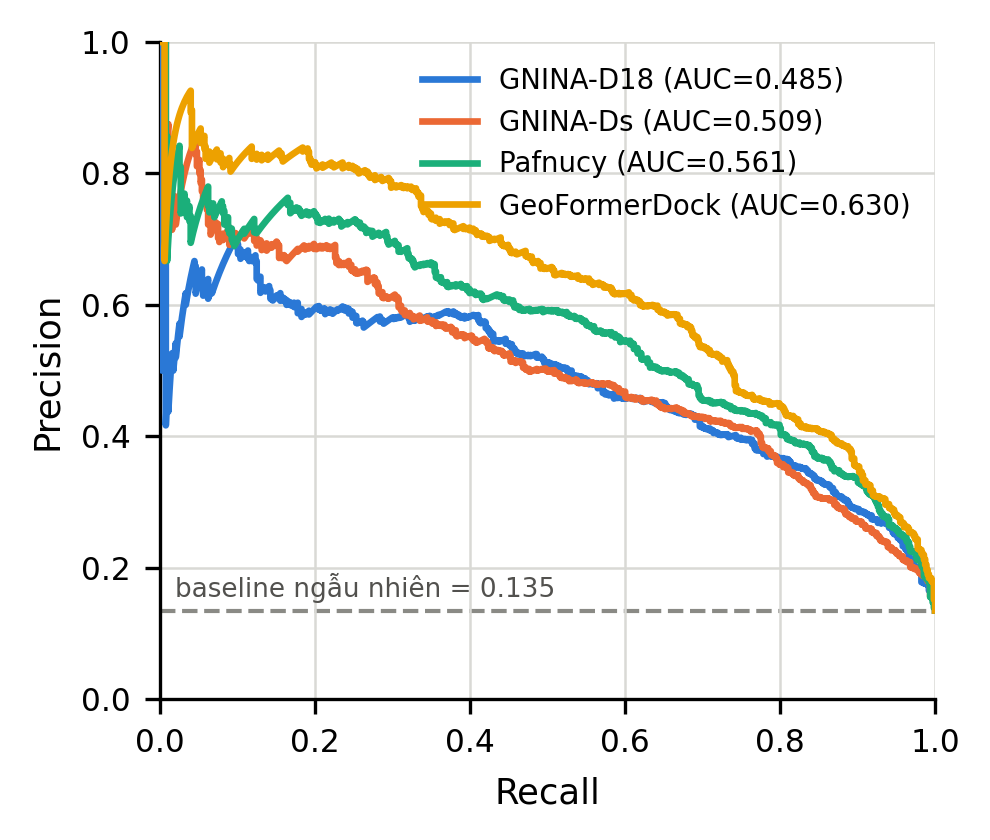
\includegraphics[width=0.43\textwidth]{figures/pr_curve.png}
    \caption{Đường cong Precision-Recall của tác vụ phân loại tư thế trên tập kiểm tra}
    \label{fig:pr_curve}
\end{figure}

Hình~\ref{fig:pr_curve} cho thấy rõ hơn hình dạng đường cong đằng sau chỉ số PR-AUC: GeoFormerDock dẫn đầu ở hầu hết dải recall, đặc biệt tại vùng recall thấp-trung bình nơi Precision thường sụt nhanh nhất do mất cân bằng lớp; bốn đường cong hội tụ gần nhau ở recall cao, cho thấy khác biệt giữa các mô hình chủ yếu nằm ở khả năng xếp hạng các mẫu dễ phân biệt hơn là các mẫu khó nhất. So sánh cặp có kiểm định (paired bootstrap, $n=2000$, $\alpha=0.05$, toàn bộ 4.618 mẫu kiểm tra) cho thấy GeoFormerDock vượt trội có ý nghĩa thống kê so với cả ba baseline trên cả Balanced Accuracy (chênh lệch trung bình $+0.040$ đến $+0.068$) và PR-AUC (chênh lệch trung bình $+0.068$ đến $+0.144$), khoảng tin cậy 95\% không chứa 0 ở toàn bộ 6 phép so sánh.

\textit{D. Phân tích đánh đổi}

\begin{figure}[H]
    \centering
    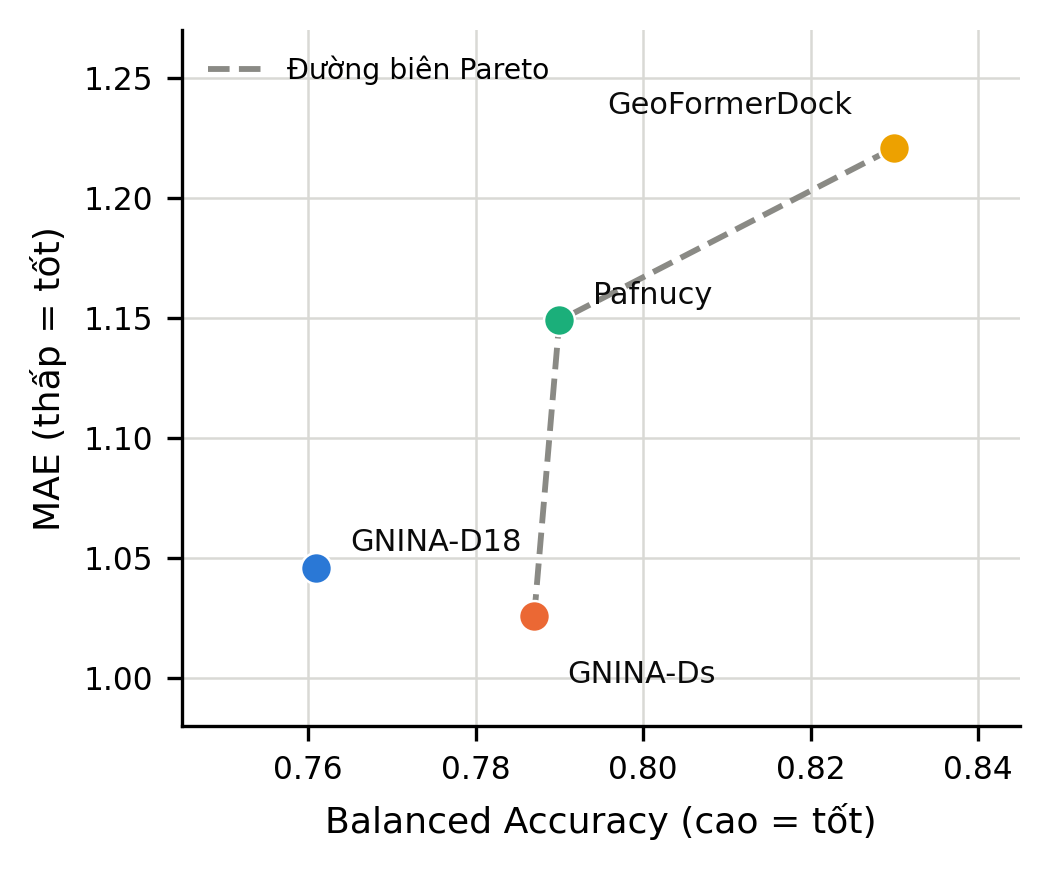
\includegraphics[width=0.45\textwidth]{figures/pareto_frontier.png}
    \caption{Đường biên Pareto giữa Balanced Accuracy (phân loại tư thế) và MAE (dự đoán ái lực) trên các mô hình so sánh.}
    \label{fig:pareto}
\end{figure}

Hình~\ref{fig:pareto} thể hiện vị trí tương đối của các mô hình trên hai mục tiêu. GeoFormerDock nằm ở cực ưu tiên phân loại tư thế, trong khi nhóm GNINA nằm ở cực ưu tiên ái lực; không mô hình nào chiếm ưu thế tuyệt đối trên cả hai trục. Đây là quan sát trên 4 điểm rời rạc chứ không phải một đường cong đánh đổi liên tục (đòi hỏi quét trọng số $w_{pose}/w_{aff}$ cho từng kiến trúc) - với chỉ 4 mô hình, việc không bị trội tuyệt đối là điều kiện dễ đạt về mặt toán học (bất kỳ mô hình nào tốt nhất ở một trục đều tự động thỏa điều kiện này), nên hiểu đây là quan sát định tính về vị trí tương đối, không phải một đường biên Pareto đầy đủ. Vị trí cụ thể của mỗi mô hình trên mặt phẳng đánh đổi không chỉ do kiến trúc quyết định: như đã nêu ở Mục IV.B, khác biệt về hàm mất mát (Gaussian NLL so với Huber) và về cân bằng lớp ở mức minibatch cũng góp phần định hình kết quả quan sát được. Với quy mô tham số nhỏ hơn 1--5 lần so với Pafnucy và GNINA Default2018, GeoFormerDock vẫn đạt Balanced Accuracy cao nhất - cho thấy sự đánh đổi này không đơn thuần là hệ quả của thiếu năng lực mô hình.
